%; whizzy chapter
% -initex iniptex -latex platex -format platex -bibtex jbibtex -fmt fmt
% $B0J>e(B whizzytex $B$r;HMQ$9$k>l9g$N@_Dj!#(B

%     Tokyo Debian Meeting resources
%     Copyright (C) 2011 Junichi Uekawa
%     Copyright (C) 2011 Nobuhiro Iwamatsu

%     This program is free software; you can redistribute it and/or modify
%     it under the terms of the GNU General Public License as published by
%     the Free Software Foundation; either version 2 of the License, or
%     (at your option) any later version.

%     This program is distributed in the hope that it will be useful,
%     but WITHOUT ANY WARRANTY; without even the implied warranty of
%     MERCHANTABILITY or FITNESS FOR A PARTICULAR PURPOSE.  See the
%     GNU General Public License for more details.

%     You should have received a copy of the GNU General Public License
%     along with this program; if not, write to the Free Software
%     Foundation, Inc., 51 Franklin St, Fifth Floor, Boston, MA  02110-1301 USA

%  preview (shell-command (concat "evince " (replace-regexp-in-string "tex$" "pdf"(buffer-file-name)) "&"))
% $B2hA|%U%!%$%k$r=hM}$9$k$?$a$K$O(Bebb$B$rMxMQ$7$F(Bboundingbox$B$r:n@.!#(B
%(shell-command "cd image201101; ebb *.png")

%%$B$3$3$+$i%X%C%@3+;O!#(B

\documentclass[mingoth,a4paper]{jsarticle}
\usepackage{monthlyreport}

% $BF|IU$rDj5A$9$k!"Kh7nJQ$o$j$^$9!#(B
\newcommand{\debmtgyear}{2011}
\newcommand{\debmtgmonth}{6}
\newcommand{\debmtgdate}{18}
% (+ (* (- 2011 2005) 12) 6 -1) started from zero
\newcommand{\debmtgnumber}{77}

\begin{document}

\begin{titlepage}
\thispagestyle{empty}
% $B%?%$%H%k%Z!<%8(B:$BJT=8I,MW$JItJ,$O:G=i$N%^%/%m$KHt$P$9$3$H(B

\vspace*{-2cm}
$BBh(B\debmtgnumber{}$B2s(B $BEl5~%(%j%"(B Debian $BJY6/2q;qNA(B\\
\hspace*{-2cm}
\includegraphics[width=210mm]{image201003/debsen.eps}\\
\hfill{}\debmtgyear{}$BG/(B\debmtgmonth{}$B7n(B\debmtgdate{}$BF|(B

% $B$3$3$O%"%C%W%G!<%H$9$k$3$H(B
\rotatebox{10}{\fontsize{32}{32} {\gt $BFC=8(B1: XXXX}}

\rotatebox{10}{\fontsize{32}{32} {\gt $BFC=8(B2: YYYY}}

\vspace*{-2cm}
\hfill{}
\includegraphics[height=6cm]{image200502/openlogo-nd.eps}
\end{titlepage}

\dancersection{Introduction}{$B>e@n(B $B=c0l(B}

\begin{multicols}{2}
 

 $B:#7n$N(BDebian$BJY6/2q$X$h$&$3$=!#$3$l$+$i(BDebian$B$N@$3&$K$"$7$rF'$_F~$l$k$H(B
 $B$$$&J}$b!"$9$G$K$I$C$W$j$H$D$+$C$F$$$k$H$$$&J}$b!"7n$K0l2s(BDebian$B$K$D$$(B
 $B$F8l$j$^$;$s$+!)(B

 Debian$BJY6/2q$NL\E*$O2<5-$G$9!#(B

 \begin{itemize}
 \item \underline{Debian Developer} ($B3+H/<T(B)$B$N0i@.!#(B
 \item $BF|K\8l$G$N!V(B\underline{$B3+H/$K4X$9$k>pJs(B}$B!W$r@0M}$7$F$^$H$a!"%"%C%W%G!<%H$9$k!#(B
 \item \underline{$B>l(B}$B$NDs6!!#(B
 \begin{itemize}
  \item $BIaCJ$P$i$P$i$J>l=j$K$$$k?M!9$,(B face-to-face $B$G=P2q$($k>l$rDs6!(B
	$B$9$k!#(B
  \item Debian $B$N$?$a$K$J$k$3$H$r8l$k>l$rDs6!$9$k!#(B
  \item Debian$B$K$D$$$F8l$k>l$rDs6!$9$k!#(B
 \end{itemize}
 \end{itemize}		

 Debian$B$NJY6/2q$H$$$&$3$H$G5f6KE*$K$O;22C<TA40w$,(BDebian Package$B$r$,$j$,$j(B
 $B$H:n$k%9!<%Q!<%O%C%+!<$K$J$C$?;Q$rLQA[$7$F$$$^$9!#>pJs$N6&M-!&3hMQ$rDL$7(B
 $B$F(B Debian$B$N:#8e$NG=F0E*$JE83+$X$NEZBf$H$7$F!"!V>l!W$H$7$F$N6u4V$rDs6!$9(B
 $B$k$N$,L\E*$G$9!#(B

\end{multicols}

\newpage

\begin{minipage}[b]{0.2\hsize}
 \definecolor{titleback}{gray}{0.9}
 \colorbox{titleback}{\rotatebox{90}{\fontsize{80}{80} {\gt $B%G%S%"%sJY6/2q(B} }}
\end{minipage}
\begin{minipage}[b]{0.8\hsize}
\hrule
\vspace{2mm}
\hrule
\begin{multicols}{2}
\tableofcontents
\end{multicols}
\vspace{2mm}
\hrule
\end{minipage}

\dancersection{$B;vA02]Bj(B}{$B4d>>(B $B?.MN(B}

$B:#2s$N;vA02]Bj$O0J2<$G$9(B:
\begin{enumerate}
 \item Debian$B;H$$$H$7$F%&%'%V%5!<%S%9$K4|BT$9$k$3$H$O2?$G$9$+!)(B
\end{enumerate}
$B$3$N2]Bj$KBP$7$FDs=P$$$?$@$$$?FbMF$O0J2<$G$9!#(B
\begin{multicols}{2}
{\small
% 
\begin{prework}{ やまだ }

最近新しいカーネルを自分でビルドすることが再び
増えてきたので、その周りでごそごそやってます。
\begin{enumerate}
\item gitでタグを打って
\item そのタグをバージョンにして
\item ビルドして
\item テストVMに導入して
\item ついでに配布サーバに設置
\end{enumerate}

の自動化とかやりました。

興味というか次に調べたいのは *-module-source な
カーネルモジュールパッケージの作り方とかDKMSの使い方。
普通のパッケージと違う点が多々ありそう。
\end{prework}

\begin{prework}{ 野首 }

ホームのMHフォルダを外から見れるようuw-imapdを入れました。インストールし
 てdebconfに答えるだけでSSL readyなimap環境になりました。
\end{prework}

\begin{prework}{ MATOHARA }

2010年11月の勉強会資料を見ながらnilfs2 をバックアップディスクに設定して
 みました.
リサイズ機能も来たようなので試してみたいです.
- [PATCH 0/4] nilfs2 resize support -- Linux NILFS Development
\url{http://www.spinics.net/lists/linux-nilfs/msg00869.html}
\end{prework}

\begin{prework}{ hattorin }

バングラデシュでDebianインストールして、ネットワークの監視系ツールをいろ
 いろとセットアップしてきました。今はDebian on SqueezeでTokyoTyrantの
 KeyValueを使い、特定の問題を早く計算するためにネットワークを使って計算
 を早くするような仕組み作りをしています。
\end{prework}

\begin{prework}{ キタハラ }

実家でプリンタの設定したり、
スキャナーの設定に失敗してました。

\end{prework}

\begin{prework}{ koedoyoshida }

最近Debianで自分がやったこと
\begin{itemize}
\item ようやく、メイン環境をSqueezeにupdate
wide-dhcpがupdateできずにはまったが、下記を見て解決。
\url{http://www.flcl.org/~takasugi/tdiary-org/?date=20061023}
\item OSC仙台に参加、出展。
\end{itemize}


\end{prework}

\begin{prework}{ emasaka }

sidでちょっとはまったとこについて、GitHubでupstreamに簡単なパッチをpull
 requestしたら、そのバージョンが数日後にsidに降りてきました。
\end{prework}

\begin{prework}{ dictoss(杉本 典充) }

最近やっていることはkfreebsdを常用していること、Debianを開発環境として
 gtkアプリを試作していること。
今後はkfreebsdでIS03を使ってテザリング、klinuxよりkfreebsdの方がおすすめ
 といえる有利分野を見つけることをやりたい。
\end{prework}

\begin{prework}{ なかおけいすけ }

興味があること:DebianLive
最近ネカフェで一夜を明かしたのですが、ネカフェのPCにコンパイラが入ってな
 くて困ったので、USBやSDカードにインストールしたDebianを持ち歩いていると
 ハッピーになれるのではないかと。
\end{prework}

\begin{prework}{ 吉野(yy\_y\_ja\_jp) }

バグレポートとDDTSS/DDTPぐらいでしょうか.
\end{prework}

\begin{prework}{ henrich }

いくつかパッケージやメッセージをルーティンの更新しました。

\end{prework}

\begin{prework}{ Osamu MATSUMOTO }

\begin{itemize}
\item インフラ,サーバ管理の自動化\\
 自動インストール,構成管理,コンフィグ投入, 監視のまでを
 ラフに綺麗に繋ぎたい。Debian的な良い組み合わせあったら教えてください。
 (cobbler+ puppet/cfengine+ nagios + なんかwebcgi的な)
\end{itemize}

\end{prework}

\begin{prework}{ まえだこうへい }
\begin{itemize}
\item *diagシリーズ(http://blockdiag.com/)のdebパッケージ化中。
\item さくらのVPSを先月契約して、lxc \& Squeezeで開発\&検証環境に。
\item あらきさんメンテナンスのDebianのAMI使ってAWSでごにょごにょと。
\end{itemize}
\end{prework}

\begin{prework}{ yamamoto }

\begin{itemize}
\item 最近Debianで自分がやったこと\\
ポチポチと公式パッケージのリビルドをしました。
\item 興味のあること\\
移植。
\end{itemize}

\end{prework}

\begin{prework}{ 岩松 信洋 }

\begin{itemize}
\item SH4 buildd のメンテ。
\item libpng15 の experimental へのアップロードとtransition作業。
\item スポンサーのパッケージチェック、アップロードなど。
\end{itemize}

\end{prework}

\begin{prework}{ 野島 貴英 }

\begin{itemize}

\item pythonでgnome-notifyめがけて再生中のデータのメタデータ送る「できるだ
 け簡単にできる」totemのプラグイン書いてみた。
 \url{http://d.hatena.ne.jp/nozzy123nozzy/20110502/1304322969}
\item sidのalsa-lib,alsa-utils,alsa-driverの解析中。
(bluetoothヘッドフォン出力相手に、alsaのみで、演奏中の音をcaptureしたい
 し、音が出る複数のアプリの音をmixして出力したいっ)
\item sidのlinux-image-2.6.39-2-686-paeにて、multi-stateなusb装置にejectコ
 マンド発行すると高い確率でOopsする件のデバッグを誰かがパッチ出すまでや
 り中。(いったい誰だ、dptぶっ壊すのは...)

\end{itemize}

\end{prework}

\begin{prework}{ 上川純一 }
\begin{itemize}
\item xslt のツールチェインをいろいろといじってみたり。
\item Javascript のコードを書いてみたり。
\end{itemize}
\end{prework}

}
\end{multicols}

\dancersection{$B:G6a$N(BDebian$B4XO"$N%_!<%F%#%s%0Js9p(B}{$B4d>>(B $B?.MN(B}
\subsection{$BEl5~%(%j%"(BDebian$BJY6/2q(B76$B2sL\Js9p(B}

% (query-replace-regexp "<.*?>" "")
% (query-replace-regexp "^[	 ]\+" "")



\dancersection{Debian Trivia Quiz}{$B4d>>(B $B?.MN(B}

$B$H$3$m$G!"$_$J$5$s(B Debian $B4XO"$NOCBj$K$*$$$D$$$F$$$^$9$+!)(BDebian$B4XO"$NOC(B
$BBj$O%a!<%j%s%0%j%9%H$r$h$s$G$$$k$HDI@W$G$-$^$9!#$?$@$h$s$G$$$k$@$1$G$O$O(B
$B$j$"$$$,$J$$$N$G!"M}2rEY$N%F%9%H$r$7$^$9!#FC$K0l?M$@$1$G$O0UL#$,$o$+$i$J(B
$B$$$H$3$m$b$"$k$+$bCN$l$^$;$s!#$_$s$J$G0l=o$KFI$s$G$_$^$7$g$&!#(B

$B:#2s$N=PBjHO0O$O(B\url{debian-devel-announce@lists.deban.org} $B$d(B \url{debian-devel@lists.deban.org}$B$KEj9F$5$l$?(B
$BFbMF$H(BDebian Project News$B$+$i$G$9!#(B

\begin{multicols}{2}
% %; whizzy-master ../debianmeetingresume201101.tex
% $B0J>e$N@_Dj$r$7$F$$$k$?$a!"$3$N%U%!%$%k$G(B M-x whizzytex $B$9$k$H!"(Bwhizzytex$B$,MxMQ$G$-$^$9!#(B
%
% $B$A$J$_$K!"%/%$%:$OJL%V%i%s%A$G:n@.$7!"$N$A$K%^!<%8$7$^$9!#5U$K%^!<%8$7(B
% $B$J$$$h$&$K$7$^$7$g$&!#(B
% (shell-command "git checkout quiz-prepare")

\santaku
{alioth.debian.org$B$,(B2$BBf$KJ,$+$l$^$7$?!#$=$N%5!<%PL>$O!)(B}
{vasks.debian.org $B$H(B wagner.debian.org}
{volks.debian.org $B$H(B don.debian.org}
{dennys.debian.org $B$H(B gusto.debian.org}
{A}
{$B$[$+$O%U%!%_%l%9$NL>A0(B}

\santaku
{$B8=:_9T$o$l$F$$$k(BPerl transition $B$N(BPerl$B%P!<%8%g%s$O!)(B}
{5.12}
{5.13}
{5.14}
{A}
{5.14$B$O$^$@(Bexperimental$B$G$9!#(B}

\santaku
{$B%W%i%$%^%j%_%i!<%5!<%P$,?7$7$/DI2C$5$l$?9q$O!)(B}
{$B%A%e%K%8%"(B}
{$BCf9q(B}
{$B%^%@%,%9%+%k(B}
{B}
{$B%A%e%K%8%"$H%^%@%+%9%+%k$O%_%i!<!#%W%i%$%^%j$G$O$J$$!#(B}

\end{multicols}

%-------------------------------------------------------------------------------
\dancersection{Debian JP $BDjNc2q5D=hM}7O$K(BXSLT$B$r;H$C$F$_$?(B}{$B>e@n=c0l(B}
%-------------------------------------------------------------------------------
\index{xsltproc}

\subsection{$BGX7J(B}

Debian$BJY6/2q$N4k2h2q5D$O(BIRC$B$rCf?4$H$7$F(B2006$BG/$K3+;O$7!"(BDebian JP $B$NDjNc2q(B
$B5D$H$7$F:#$bB3$$$F$$$^$9!#Ev=i$O7hDj;v9`$J$I$K$D$$$F%F%-%9%H%U%!%$%k$G$^(B
$B$H$a$k$H$$$&7A$r$H$C$F$$$^$7$?!#(BIRC$B$G$h$j8zN($h$/5DO@$9$kJ}K!$rLO:w$7$?7k(B
$B2L!"5DO@$7$J$,$i5D;vO?$rJT=8$9$k$H$$$&%9%?%$%k$,3NN)$7!"$=$l$r;Y1g$9$k$?(B
$B$a$N%D!<%k$r@0Hw$7$^$7$?!#(B

$B5D;vO?$N%=!<%9$O5DD9$,(BXML$B$G5-=R$7$F!"5DO@$N:GCf$OHsF14|$K(BJavascript$B$GFb(B
$BMF$,99?7$5$l$k(BHTML$B%U%!%$%k$rMxMQ$7$^$9(B($B@$4V0lHL$G$O(BAJAX$BE*$H$G$b$h$V$h$&(B
$B$G$9(B)$B!#(B

IRC$B$G$NDjNc2q5D$N5DO@$NA0$H8e$K$O5D;v0F$H5D;vO?$r%a!<%j%s%0%j%9%H$K$*$/$C(B
$B$F$$$^$9!#%a!<%j%s%0%j%9%H$K%a!<%k$G$J$2$k:]$K$O!"%F%-%9%H%U%)!<%^%C%H$K(B
$B$7$FAw$C$F$$$^$9!#(B

$B$"$H!"8=:_MQES$,$J$$$G$9$,!"(B\LaTeX $B7PM3$G(BPDF$B7A<0$G$N=PNO$J$I$b%5%]!<%H$7(B
$B$F$$$^$9!#(B

$B8=:_$N<BAu$ONr;KE*$J7P0^$K$h$j(BXML$B$N=hM}7O$O(B dancer-xml $B%i%$%V%i%j$H(B
boost$B$rMxMQ$7$?(BC++$B$N%W%m%0%i%`$K$J$C$F$$$^$9!#(B
dancer-xml\cite{dancer-xml} $B$O(B10$BG/A0$K<c5$$N$$$?$j$G<BAu$7$?(BXML$BIwJ8=q$N%Q!<(B
$B%5!<$G$9!#0lIt%(%s%F%#%F%#!<$^$o$j$J$I??LLL\$K<BAu$7$F$$$J$$ItJ,$,$"$k$?(B
$B$a!"E,@Z$J=hM}$,$J$5$l$F$$$J$$$3$H$,$"$j$^$9$,!"KM$N9%$_$K6uGrJ8;z=hM}$O(B
$B%A%e!<%K%s%0$5$l$F$*$j2wE,$G$9!#(B

$B:#2s$ND)@o$O!"FH<+(BC++$B%3!<%I%Y!<%9$r(BXSLT$B$K$N$;BX$($F$_$k$H$$$&D)@o$G$9!#(B

\subsection{XSLT$B$C$F$I$s$J8@8l(B?}

XSLT$B$O(BXML$B$G5-=R$9$k(BXML$B=hM}8@8l$G$9!#(B

XSLT$B4k2h$K$O(B1999$BG/$K:vDj$5$l$?(BXSLT 1.0 $B$H!"(B2007$BG/$4$m$N(BXSLT 2.0$B$,$"$j$^$9!#(B
$B:#2s$O<BAu$,==J,8O$l$F$$$k$H;W$o$l$k(B XSLT 1.0 $B$N=hM}7O$r:NMQ$7$^$7$?!#8e(B
$B$G8+$?$H$3$m(BDebian$B$GMxMQ$G$-$k(Bxslt 2.0$B$N<BAu$H$7$F$O(B libsaxonb-java$B$,$"$k(B
$B$h$&$G$9$,!":#2s$OD4::$7$F$$$^$;$s!#(B

$B%W%m%0%i%`$r=q$/$H$-$K$9$Y$-J8=q$H$7$F$O!"(BXSLT$B<+BN$N(B1999$BG/$K:vDj$5$l$?5,(B
$B3J(B\cite{xslt1999}$B$H!"(BXSLT$B$NCf$G5-=R$G$-$k(BXPATH$B$N5,3J(B\cite{xpath1999}$B$r;2(B
$B>H$9$k$H$h$$$G$7$g$&!#(B

XSLT$B$@$1$G$O$"$^$j9bEY$J%W%m%0%i%_%s%0$O$G$-$J$$$s$8$c$J$$$+$H;W$o$l$k$+(B
$B$b$7$l$^$;$s$,!"4X?t7?8@8l$H$7$F==J,$J5!G=$rDs6!$G$-$kNO$O$"$k$h$&$G$9(B
\cite{fxslt2003}$B!#(B

\subsection{Debian $B$GMxMQ2DG=$J(B XSLT$B=hM}7O(B}

Debian$B$GI}9-$/;H$o$l$F$$$F0BDj$7$F$$$k$H$*$b$o$l$k$N$H!"4JC1$KMxMQ$G$-$k(B
$B$H$$$&M}M3$G=hM}7O$H$7$F(B xsltproc $B$r:NMQ$7$^$7$?!#(B

Debian $B$G$N(B xsltproc $B$N%$%s%9%H!<%k$O4JC1(B
\begin{commandline}
$ apt-get install xsltproc
\end{commandline}
%$

$B%3%^%s%I%i%$%s$G0J2<$N$h$&$K<B9T$9$k$HI8=`=PNO$K=hM}:Q$_(BXML$B$,=PNO$5$l$^$9!#(B

\begin{commandline}
$ xsltproc [$B%9%?%$%k%7!<%H(B] [$B=hM}$9$k(BXML$B%U%!%$%k(B]
\end{commandline}
%$

\subsection{$B6qBNNc(B:HTML}

$B$=$l$G$O!"(BHTML$B=PNO$N>l9g$r8+$F$_$^$7$g$&!#(B
\url{meetinglog:html.xsl}$B$G$9!#(B
XML$BJ8=q$+$i(BHTML$BJ8=q$r@8@.$9$k$K$O$=$l$J$j$KJXMx$J8@8l$G$9!#(B

$BA0H>$N%3!<%I$r$=$N$^$^7G:\$7$^$9!#(B
$B$3$l$O!"(BXML$B%I%-%e%a%s%HA4BN$K%^%C%A$9$k%k!<%k$r5-=R$7$O$8$a$k$^$G$NItJ,(B
$B$G$9!#(B
XML$BL>A06u4V$H$7$F!"%G%U%)%k%H$r(BHTML$B!"(Bxsl$B$r(Bxslt$B$NL>A06u4V$K3d$jEv$F$F$$$^(B
$B$9!#(B

xml:output $B$G=PNO7A<0$r(BHTML$B$H;XDj$9$k$3$H$G(BXML$B%X%C%@$,=PNO$5$l$:$KJXMx$G(B
$B$9!#(B

\begin{commandline}
<?xml version="1.0"?>
<!DOCTYPE xsl:stylesheet>
<xsl:stylesheet version="1.0"
  xmlns:xsl="http://www.w3.org/1999/XSL/Transform"
  xmlns="http://www.w3.org/1999/xhtml">
  <xsl:output method="html" />
  <xsl:template match="/">
    <html>
      <head>
\end{commandline}

$BB>$K(BXSLT$B$NFCD'E*$J$H$3$m$O!"(Bvalue-of$B!!$GCM$r$H$C$F$-$F$$$^$9!#(BXPATH
$B$N=q<0$G;XDj$7$F$$$^$9$,!"(B
\begin{commandline}
	<h1><xsl:value-of select="meetinglog/head/title"/></h1>
\end{commandline}

$B$O!"(BXML$BJ8=q$N0J2<$N$h$&$J%(%l%a%s%H$KF~$C$F$$$kCM$rCj=P$7$^$9!#(B
\begin{commandline}
 <meetinglog>
   <head>
     <title>$B%?%$%H%k(B</title>
   </head>
 </meetinglog> 
\end{commandline}

$B5D;vO?$N>l9g$N%a%$%s%k!<%W$O!"3F5D;v$KBP$7$F$N=hM}$G$9!#(B
xsl$B$N(Bxsl:for-each$B$r$D$+$$!"(BXML$B$N%(%l%a%s%H%N!<%I$N?t$@$1%k!<%W$7$^$9!#(B
HTML$B%?%0$O$=$N$^$^=PNO$5$l$^$9$,!"$b$7(BHTML$B$N%"%H%j%S%e!<%H$J$I$r(BXSLT$B$G@8(B
$B@.$7$?$$>l9g$O!"(Bxsl:element $B$r;H$C$F%(%l%a%s%H$r@8@.$7$^$9!#(B

position()$B4X?t$O8=:_$N%(%l%a%s%HHV9f$r$/$l$k$N$G$3$&$$$&>l9g$KJXMx$G$9!#(B

\begin{commandline}
           <xsl:for-each select="meetinglog/body">
	      <tr>
		<th>
		  <xsl:element name="a">
		    <xsl:attribute name="href">#gian<xsl:value-of select="position()" /></xsl:attribute>
		  </xsl:element>
		  $B5D0F(B<xsl:value-of select="position()" />
		</th>
		<td class="bodytitle">
		  <xsl:value-of select="./title" />
		</td>
 ....
 </xsl:for-each> 
\end{commandline}

\subsection{$B6qBNNc(B:Text$B=PNO(B}

Text$B=PNO$N>l9g$b$_$F$_$^$7$g$&!#(B
\url{meetinglog:txt.xsl}
$B%F%-%9%H=PNO$r$7$h$&$H$7$O$8$a$k$H<c436l$7$/$J$C$F$-$^$9!#$G$-$J$$$o$1$G(B
$B$O$J$$$N$G$9$,!"6uGrJ8;z$N=hM}$N%k!<%k$rKM$,$$$^$$$AM}2r$G$-$F$$$J$$$N$H!"(B
$B%3!<%I$,$=$N$^$^%F%s%W%l!<%H$H$7$F=PNO$5$l$k$N$G%$%s%G%s%F!<%7%g%s$,E,@Z(B
$B$K$G$-$J$$$N$,$D$i$$$H$3$m$G$9!#(B

xsl:output $B$G=PNO$,%F%-%9%H7A<0$G$"$k$H;XDj$9$k$H(BXML$B%X%C%@$,=PNO$5$l$:JX(B
$BMx$G$9!#(B

$B%X%C%@ItJ,$G!"Kh2s(B xsl:text $B$G2~9T$J$I$rF~NO$9$k$N$,LLE]$J$N$G!"(BENTITY $B$r(B
$BDj5A$7$F>JN,$G$-$k$h$&$K$7$F$$$^$9!#$3$N5-K!$,@5$7$$$N$+$I$&$+$OITL@$G$9!#(B

\begin{commandline}
<?xml version="1.0"?>
<!DOCTYPE xsl:stylesheet [
<!ENTITY space  "<xsl:text xmlns:xsl='http://www.w3.org/1999/XSL/Transform'> </xsl:text>">
<!ENTITY indent "<xsl:text xmlns:xsl='http://www.w3.org/1999/XSL/Transform'>  </xsl:text>">
<!ENTITY cr     "<xsl:text xmlns:xsl='http://www.w3.org/1999/XSL/Transform'>
</xsl:text>">]>
  <xsl:stylesheet version="1.0"
    xmlns:xsl="http://www.w3.org/1999/XSL/Transform"
    xmlns="http://www.w3.org/1999/xhtml">
  <xsl:output method="text" />
  <xsl:template match="/">
    <xsl:text>-----------------------------------------------------------------------
$B35MW(B
-----------------------------------------------------------------------
\end{commandline}

$BK\J8$N%3%"$H$J$kK\J8$NFbMF$G$9$,!"FI$a$?$b$N$G$O$J$$$G$9!#(B
$BG:$s$@$H$3$m$H$7$F$O!"J8>O$,6uGr$+$I$&$+%A%'%C%/$9$k$N$K(B
string-length(normalize-space())$B$r$D$+$C$F$$$F!"$=$l$,$$$^$$$A$?$@$7$$$N(B
$B$+$I$&$+<+?.$,$J$$$H$3$m!#(B

\begin{commandline}
    <xsl:for-each select="meetinglog/body">
-----------------------------------------------------------------------
[<xsl:value-of select="position()" />.&space;<xsl:value-of select="./title" />]
-----------------------------------------------------------------------

$BL\E*(B: &cr;<xsl:value-of select="./aim" />&cr;
&cr;<xsl:if
 test="string-length(normalize-space(./previous))>1"
 >$BA02s$^$G$N7P0^(B:&cr;<xsl:value-of select="./previous"
 disable-output-escaping="yes" />&cr;&cr;</xsl:if>
<xsl:if test="string-length(normalize-space(./discussed))>1"
 >$B5DO@(B:&cr;<xsl:value-of select="./discussed"
 disable-output-escaping="yes" />&cr;&cr;&cr;
</xsl:if>
</xsl:for-each>
\end{commandline}

$B;DG0$J$,$i(BC++$B$G<BAu$7$F$$$?J8;z$r%a!<%k$N(B70$BJ8;zI}$/$i$$$K$-$l$$$K$^$H$a(B
$B$k$H$$$&%m%8%C%/$,7gMn$7$F$$$^$9!#$a$s$I$/$5$9$.$k!#(B

\subsection{$B6qBNNc(B:\LaTeX}

\LaTeX $B=PNO$r$_$F$_$^$7$g$&!#(B
\url{meetinglog:latex.xsl}

$B%X%C%@ItJ,$O$I$&$<(B\LaTeX{}$B$N%X%C%@$J$N$H2?EY$b$G$F$-$F$$$k$N$G%a%$%s%k!<%W(B
$B$@$1!#(B
\begin{commandline}
    <xsl:for-each select="meetinglog/body">

      \discussion{<xsl:value-of select="./title" />}{<xsl:value-of
 select="./aim" />}{<xsl:value-of
 select="translate(./previous,'#&amp;','--')"
 disable-output-escaping="yes" />}{<xsl:value-of
 select="translate(./discussed,'#&amp;','--')"
 disable-output-escaping="yes" />}
    </xsl:for-each>
\end{commandline}

$B8D?ME*$J46A[$G$9$,!"<+J,$G=q$$$F$*$-$J$,$i8e$GFI$_JV$95$NO$,J($-$^$;$s!#(B

$B8=:_<BAu$G$-$F$$$J$$E@$H$7$F!"(B\LaTeX{}$B$G;H$($J$$J8;zNs(B\verb!#<>&!$B$J$I$NJ8(B
$B;zNs$N%(%9%1!<%W$,$"$j$^$9!#:#$O%O%$%U%s$KJQ99$7$F$*Cc$rBy$7$F$$$^$9!#(B

XPATH$B$K$OJ8;zNsCV49$N$?$a$N(Btransform()$B4X?t$,$"$j$^$9$,!"0lJ8;z$r0lJ8;z$KCV49(B
$B$9$k$3$H$7$+$G$-$^$;$s!#:#2s9T$$$?$$$N$O0lJ8;z$rJ#?tJ8;z$KCV49$9$k$3$H$J(B
$B$N$G$=$l$G$O5!G=$,IT==J,$G$9!#(B

\subsection{$B2>$NDjNLE*$JHf3S(B}

$B8=>u$9$Y$F$N5!G=$r$*$-$+$($F$$$k$o$1$G$O$J$$$N$G!"BEEv$JHf3S$G$O$J$$$G$9(B
$B$,!"(BC++$B$N=hM}$H(BXSLT$B$N%3!<%I$NHf3S$r$7$F$_$k$H(B
(\ref{tab:xsltcxximplementationdiff})$B!"(B
XSLT$B$N$[$&$,9T?t$O>/$J$$$3$H$,$o$+$j$^$9!#(B

\begin{table}[ht]
 \caption{lines of code for each implementation}
 \label{tab:xsltcxximplementationdiff}
\begin{center}
  \begin{tabular}{|c|c|c|}
 \hline
 & c++ & xslt \\
 \hline
 txt & 151 & 53\\
 html & 157 & 99 \\
 latex(PDF) & 158 & 87 \\
 \hline
 \end{tabular}
\end{center}
\end{table}

\subsection{$B7kO@(B}

XSLT$B$r;H$&$3$H$G%a%s%F%J%s%9$9$k9T?t$O>/$J$/$J$j$^$9!#$7$+$7!"(BXPATH /
XSLT $B$K$h$jDs6!$5$l$F$$$k5!G=$,@)8B$5$l$F$$$k$?$a!"$=$NCf$G<B8=$G$-$J$$$b(B
$B$N$K$D$$$F$OFq$7$$H=CG$rGw$i$l$^$9!#(B

$B4hD%$l$P@)8B$O2sHr$G$-$k$1$I$I$3$^$G2sHr$9$k$+!"G:$^$7$$$H$3$m$G$9!#(B

\begin{thebibliography}{0}
 \bibitem{fxslt2003} Dimitre Novatchev, ``Functional programming in XSLT
	 using the FXSL library,'' Extreme Markup Languages 2003.
 \bibitem{xslt1999} James Clark, ``XSL Transformations (XSLT)
	 Version 1.0,'' W3C Recommendation 16 November 1999.
	 \url{http://www.w3.org/TR/xslt}
 \bibitem{xpath1999} James Clark, Steve DeRose, ``XML Path Language
	 (XPath) Version 1.0,'' W3C Recommendation 16 November 1999.
	 \url{http://www.w3.org/TR/xpath/}
 \bibitem{dancer-xml} Junichi Uekawa, ``dancer-xml - Simple
	 non-comformant XML parsing library,'' 2000.
	 \url{http://www.netfort.gr.jp/~dancer/software/dancer-xml.html}
\end{thebibliography}


%-------------------------------------------------------------------------------
\dancersection{XXXX}{$B>e@n=c0l(B}
%-------------------------------------------------------------------------------
\index{fuga}

\printindex

\cleartooddpage

\vspace*{15cm}
\hrule
\vspace{2mm}

\includegraphics[width=2cm]{image200502/openlogo-nd.eps}
\noindent \Large \bf Debian $BJY6/2q;qNA(B\\
\noindent \normalfont \debmtgyear{}$BG/(B\debmtgmonth{}$B7n(B\debmtgdate{}$BF|(B \hspace{5mm}  $B=iHGBh(B1$B:~H/9T(B\\
\noindent \normalfont $BEl5~%(%j%"(B Debian $BJY6/2q(B $B!JJT=8!&0u:~!&H/9T!K(B\\
\hrule

\end{document}
